\subsection{課題説明}
3種類の連続関数$y=x^2$、$z=x^2+y^2$、$y=-x \times sin(x)$について、
最急降下法の適用を通して探索挙動を観察した。
以下ではまず共通部分である最急降下法の探索手続きについて、
フローチャートを用いて解説する。
その後、3種類の関数毎にプログラムの変更箇所、
観察意図観察方法、観察結果、考察について説明する。
\subsection{Level 2共通部分}

\subsubsection{探索の手続きとフローチャート(共通部分)}
\begin{figure}[htbp]
  \begin{center}
    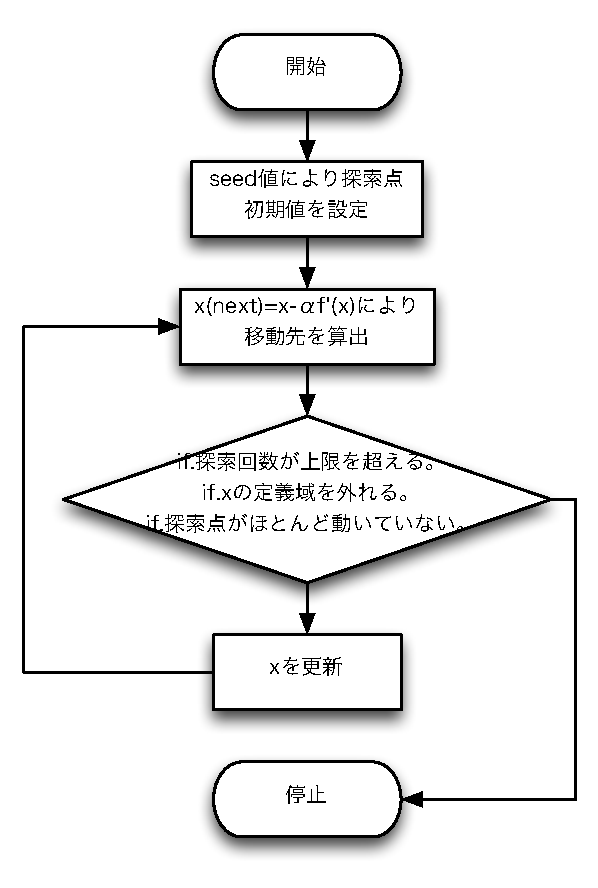
\includegraphics[clip,width=10.0cm]{./figs/tonal1.pdf}
    \caption{探索手続きのフローチャート}
 \end{center}
\end{figure}
\newpage
